
\section{Diffraction of Light}

Name \rule{2.0in}{0.1pt}\hfill{}Section \rule{1.0in}{0.1pt}\hfill{}Date
\rule{1.0in}{0.1pt}

\textbf{Objective}

To investigate how the interference and diffraction of light waves
combine to form a distinctive pattern and how that pattern can be
used to measure the size of an object.

\textbf{Introduction}

In this laboratory you will investigate the interference and diffraction
of light produced by a laser beam passing through a set of narrow,
adjacent slits. When light passes through a set of slits, each opening
acts as an independent source of waves that can overlap one another
to produce a distinctive pattern of bright and dark spots on a screen.
The position of the bright spots depends on the separation of the
adjacent slits and the wavelength of the incident light. In addition,
diffraction produced by the individual slits modifies the intensity
of each spot. To perform the following activities you will need:

\begin{itemize}
\item Basic optics diode laser
\item Optical bench with rotary motion sensor
\item Phototransistor for measuring light intensity (mounted on rotary motion sensor)
\item ``Multiple Slit Set'' slit accessory
\item ``Single Slit Set'' slit accessory
\item {\it Pasco} 550 Interface.
\end{itemize}
You can measure this interference/diffraction pattern with the setup
shown below. A phototransistor is seated behind the narrow opening on top
of the metal mount. The phototransistor can translate the intensity
of the light falling on it into a voltage signal that can be read
by the computer. In addition, the phototransistor can be moved back and
forth on a rotary motion sensor that measures the position of the 
mount.
These two signals can be combined to
make a graph of the intensity as a function of position.

\vspace{0.3cm}
%{\centering \resizebox*{0.75\textwidth}{!}{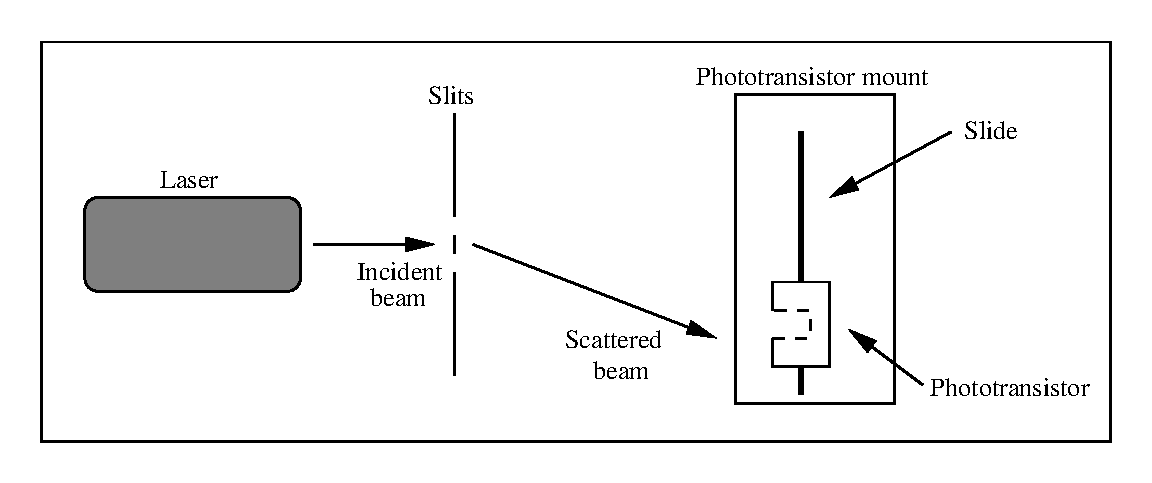
\includegraphics{interference_of_light_fig_1.eps}} \par}
\begin{center}
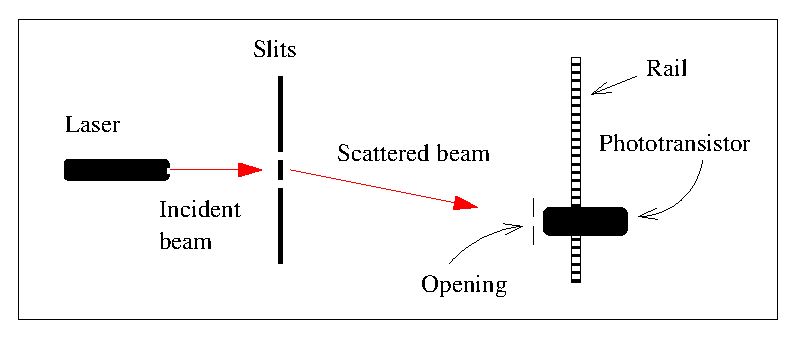
\includegraphics{diffraction/diffraction_of_light_fig1b.eps}
\index{color page}
\end{center}
\vspace{0.3cm}

{\centering \textbf{Fig. 1}. View of diffraction apparatus from above.\par}

In this unit you will  pass light of known wavelength through slits 
and use the diffraction pattern to determine the size of the individual
slit through which the light passed.

\newpage

\textbf{Intensity of Interference }

For light that passes through two very narrow slits one can calculate
a theoretical expression for the interference pattern that would be
produced in such a situation. The expression is 

%\begin{displaymath} I_{int} = 4I_0 cos^2 (\frac {\pi d} {\lambda} \sin \theta ) \end{displaymath}
\begin{equation} I_{int} = 4I_0 cos^2 \left (\frac {\pi d} {\lambda} \sin \theta \right ) \end{equation}

where $I_{int}$ is the intensity of the light at the phototransistor,
$I_{0}$ is the maximum intensity of the incident light, d is
the slit separation, \( \theta  \) is the angular position of the
scattered light relative to the incident beam, and \( \lambda  \)
is the wavelength of the light. This expression has a characteristic
shape shown below. We will compare this prediction of {}``pure''
interference (without diffraction effects) with the measured pattern
in the next activity.

\vspace{-0.10cm}
{\centering 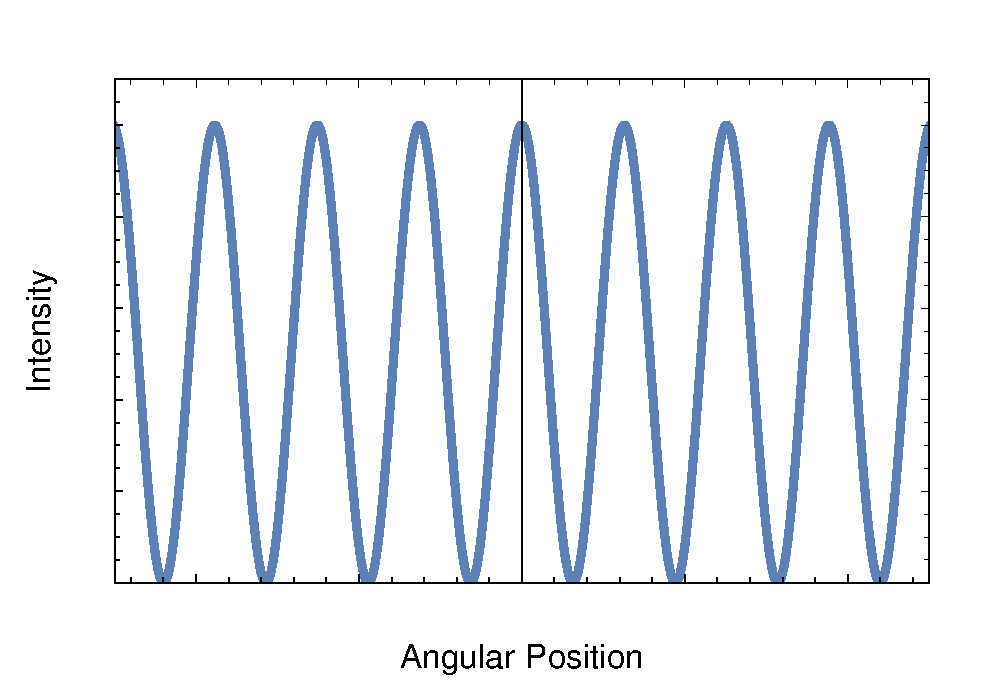
\includegraphics[height=2.75in]{diffraction/diffractionFig1.eps} \par}
\index{color page}
\vspace{0.1cm}

{\centering \textbf{Fig. 2}. Intensity distribution of pure interference.\par}

\textbf{Activity 1: The Intensity of the Interference of Light }

(a) You are now ready to turn on the laser. DO NOT LOOK DIRECTLY INTO
THE BEAM OR POINT THE LASER CARELESSLY ABOUT THE ROOM. Turn on the
laser and you should see the bright red spot of the beam striking
the rotary motion sensor assembly. On the ``Multiple Slit Set'' accessory, 
select a double slit of width 0.04 mm and separation 0.125 mm marked by the number “2”. 
Rotate the 
wheel so that the double slit is at the center of the opening.
You can rotate the wheel with the slits AND rotate where the slit wheel is mounted
on the plastic frame. Rotate both so that when you click the frame onto the optical bench, the double slit that
you want is at the center of the opening, with the slits oriented vertically and the laser beam centered right on
it. You should now see the “interference pattern” consisting of a series of bright spots a few millimeters apart,
on the white screen in front of the light sensor.

(b) On the light sensor itself, set the small gain switch to “100” (highest sensitivity). Rotate the aperture wheel
in front of the sensor to the position marked “3”. (Wider gaps let in more light; narrower gaps measure light
at a more precisely defined location.) Also check that the sensor is exactly perpendicular to the incident beam;
adjust its mounting if necessary.

(c) Position the double slit about 70 cm from the phototransistor mount. Adjust 
the laser beam direction so that it falls on the double slit you have selected. 
(There are two adjustment screws on the back of the laser.) 
You should see the interference pattern on the phototransistor mount. 
Use the markings on the optical bench to measure the distance from the slits
to the phototransistor case.
Record your value here.
\vspace{10mm}

(d) Position the phototransistor mount so the interference pattern
is at the same height as the opening in the center of the phototransistor mount. 
The phototransistor is mounted behind this hole. 
To make accurate measurements it is important to carefully determine the geometry of your setup. 
Check to see if the slits and the phototransistor mount are perpendicular to the incident
laser beam.  You want to make sure the phototransistor can {}``see'' as many
bright spots as possible. Carefully slide the phototransistor mount 
back and forth to make sure that it stays centered on the interference pattern. 
Then set it at one side of the pattern to begin the experiment.

(e) Open the file {\it Interference.cap} in the {\it Phys132} folder. 
When you are ready, click {\it Record} and slowly move the
detector assembly from one side of the bright spots to the other by rotating the turn wheel on the rotary motion
sensor. Move carefully and take about ten seconds to complete the motion. As you move it, the computer screen
should show a graph of the intensity reading versus the position reading. Click {\it Stop} when you’re done. The
graph, called the interference pattern, should be a symmetric pattern of distinct peaks. Consult your instructor
if your setup isn’t working.
Make a hardcopy of this graph and attach it to this unit.

(f) In the space below, draw a good graph showing your interference pattern. Be sure to label your axes!
\vspace{25mm}

(g) Is the spacing between the intensity peaks constant? Is the intensity
of each peak the same? Does it appear that any peaks are missing?
How does the measured intensity spectrum compare with the one predicted
for {}``pure'' interference discussed above? What is different?
What is the same?
\vspace{30mm}

(h) Measure and record the Position Reading and Intensity Reading
of each peak in the table below or in Excel and save it for later (see Appendix D).
Use the
{\it Coordinates/Delta Tool} to accurately read off the peak positions by clicking on the
appropriate button along the top of the graph. A set of cross-hairs will appear on the
plot. Grab the cross-hairs by clicking on them and dragging them to the point you want
to measure.
The coordinates will be printed by the cross-hairs.
Turn off the laser when you are finished.
We will return to these results in Activity 4.

\vspace{0.3cm}
{\centering \begin{tabular}{|c|c|}
\hline 
Position Reading (m)&
Intensity Reading (\%)\\
\hline
\hline 
&
\\
\hline 
&
\\
\hline 
&
\\
\hline 
&
\\
\hline 
&
\\
\hline 
&
\\
\hline 
&
\\
\hline 
\end{tabular}
\quad
\begin{tabular}{|c|c|}
\hline 
Position Reading (m)&
Intensity Reading (\%)\\
\hline
\hline 
&
\\
\hline 
&
\\
\hline 
&
\\
\hline 
&
\\
\hline 
&
\\
\hline 
&
\\
\hline 
&
\\
\hline 
\end{tabular}}
\vspace{0.3cm}


\textbf{Activity 2: The Diffraction of Light} 

(a) We'll now measure the diffraction of light from a single slit.
Replace the ``Multiple Slit Set'' accessory with the ``Single Slit Set'' accessory
and select a single slit of width 0.04 mm.
Notice the width of the slit here is the same as in Activity 1.
Rotate the wheel so that the single slit is at the center of the opening.
You can rotate the wheel with the slits AND rotate where the slit wheel is mounted
on the plastic frame. 
Rotate both so that when you click the frame onto the optical bench, the single slit that
you want is at the center of the opening, with the slits oriented vertically and the laser beam centered right on
it. You should now see the “diffraction pattern” consisting of a set of wide, bright spots 
on the white screen in front of the light sensor.

(b) Check that your apparatus is set up the same way is was for Activity 1 (gain switch on the phototransistor,
aperture in front of the sensor, geometry of the setup).

(c) Position the single slit about 70 cm from the phototransistor mount. Adjust 
the laser beam direction so that it falls on the double slit you have selected. 
(There are two adjustment screws on the back of the laser.) 
You should see the diffraction pattern on the phototransistor mount. 
Use the markings on the optical bench to measure the distance from the slits
to the phototransistor case.
Record your value here.
\vspace{10mm}

(d) Position the phototransistor mount so the interference pattern
is at the same height as the opening in the center of the phototransistor mount. 
The phototransistor is mounted behind this hole. 
To make accurate measurements it is important to carefully determine the geometry of your setup. 
Check to see if the slits and the phototransistor mount are perpendicular to the incident
laser beam.  You want to make sure the phototransistor can {}``see'' as many
bright spots as possible. Carefully slide the phototransistor mount 
back and forth to make sure that it stays centered on the interference pattern. 
Then set it at one side of the pattern to begin the experiment.

(e) Open the file {\it Interference.cap} in the {\it Phys132} folder. 
When you are ready, click {\it Record} and slowly move the
detector assembly from one side of the bright regions to the other by rotating the turn wheel on the rotary motion
sensor. Move carefully and take about ten seconds to complete the motion. As you move it, the computer screen
should show a graph of the intensity reading versus the position reading. Click {\it Stop} when you’re done. The
graph, called the diffraction pattern, should be symmetric about the large, central peak. Consult your instructor
if your setup isn’t working.
Make a hardcopy of this graph and attach it to this unit.

(f) In the space below, draw a good graph showing your interference pattern. Be sure to label your axes!
\vspace{25mm}

(g) When you are satisfied with the quality of your spectrum record the 
position of of the central peak and the minima (dark spots) on either side of the central peak.
Use the {\it Coordinates/Delta Tool} 
described in {\it Appendix A} to accurately read off 
the peak positions by clicking on the appropriate button along the top of the 
graph. A set of cross-hairs will appear on the plot. Grab the cross-hairs by 
clicking on them and dragging them to the point you want to measure.
The coordinates will be printed by the cross-hairs.
Turn off the laser when you are finished.
\vspace{25mm}

\newpage

(h) How would you calculate the angle between the central maximum and the first 
minimum on each side of it? Write down your formula here and list the quantities in the expression.
\vspace{25mm}

(i) Use the formula above and your your measurements in (g) to calculate the
angle between the central peak and the two minima.
Record your results here.
What is the angular width of the central peak?
\vspace{25mm}


% (j) Collect the results for the angular width from the other teams in class
% and calculate the average and standard deviation. Record the result here.
% Are your results consistent with the class results? Why or why not?
% We'll use these measurements in the next Activity.
% \vspace{40mm}

\textbf{Activity 3: Intensity of Diffraction} 

Applying the same theoretical techniques that were applied to interference
(see equation above) one can derive a prediction for the intensity
pattern due to diffraction of light passing through a single slit.
The result is 

\begin{equation} I_{diff} = I_m \left (\frac {\sin (\frac {\pi a} {\lambda} \sin \theta)} {\frac {\pi a} {\lambda} \sin \theta} \right )^2 \end{equation}

where $a$ is the size of the single slit, \( \theta  \) is the angular
position of the phototransistor relative to the incident beam, $I_{m}$
is the maximum intensity at the center of the diffraction pattern,
and \( \lambda  \) is the wavelength of the light. The shape of this
intensity distribution is shown in Figure 3.

\vspace{-0.1cm}
{\centering 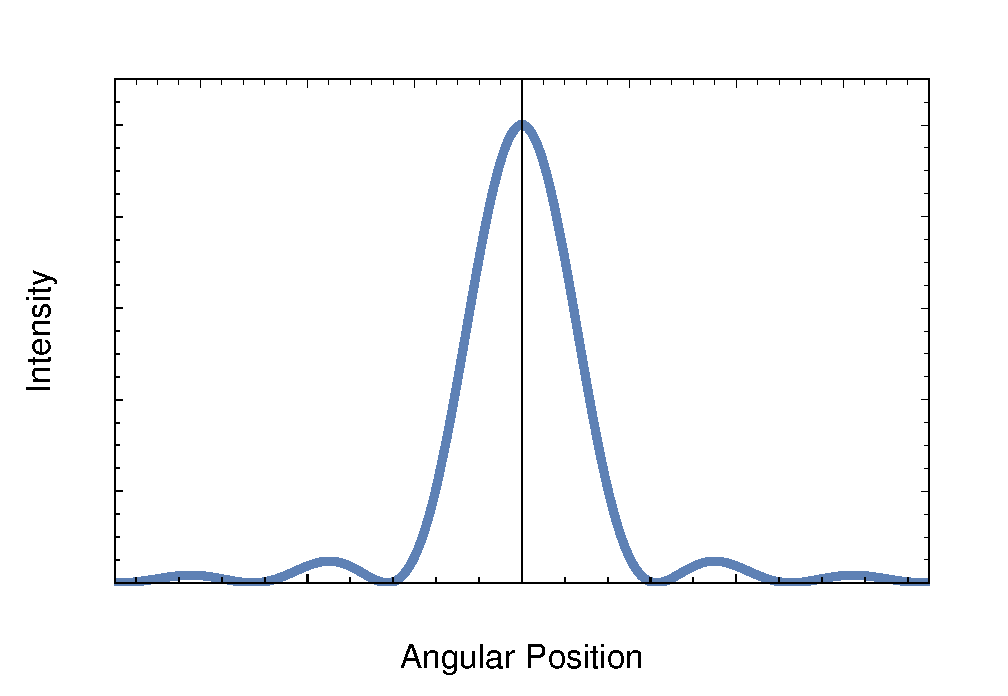
\includegraphics[height=2.75in]{diffraction/diffractionFig2.eps} \par}
\index{color page}
\vspace{0.1cm}

{\centering \textbf{Fig. 3}. Intensity distribution of diffraction
from a single slit.\par}

\newpage

(a) The figure above shows the diffraction pattern has a central maximum
with a series of points where the intensity goes to zero at positive
and negative angles. At what angle $\theta$  is the expression for 
the intensity in the equation above equal to zero? Give your answer
in terms of $a$, $\lambda$ and any other constants.
\vspace{20mm}

(b) Using the result of part (a), what is the angular position of
the minima on either side of the central maximum
in terms of $a$, $\lambda$ and any other constants?
\vspace{20mm}

(c) Finally, generate an expression for the angular width of the central
maximum in terms of $a$, \( \lambda  \), and any other constants you
need.
\vspace{30mm}

(d) Using the known wavelength of the laser $\lambda$, $L$ the distance from
the slit to the sensor, and the $a$ the size of the slit calculate the angular 
width of the central peak.
Does it agree with your measurement of the angular width in Activity 2.i?
What is your percent difference?
\vspace{30mm}

(e) Collect the results for the angular width from the other teams in class
and calculate the average and standard deviation. Record the result here.
Are your results consistent with the class results? Why or why not?
\vspace{40mm}

\textbf{Combining Interference and Diffraction}

By now you may have realized that your measured intensity distribution
from Activity 1
does not  agree with the distribution predicted by {}``pure''
interference as represented by Equation 1 and Figure 2. When
light passes through a pair of slits diffraction occurs at each individual
slit and casts the characteristic pattern described by  
Equation 2. At the same time there is interference between the light
from different slits that creates an interference pattern described
by Equation 1. The net effect is a multiplication of these
two equations to yield 

\begin{equation} I_{total} = I_m \cos^2 (\frac {\pi d} {\lambda} \sin \theta ) (\frac {\sin (\frac {\pi a} {\lambda} \sin \theta)} {\frac {\pi a} {\lambda} \sin \theta} )^2 \end{equation}

where $I_{m}$ is the intensity of the central maximum, \( \theta  \)
is the position of the phototransistor, $d$ is the separation of the
slits, $a$ is the size of an individual slit, and \( \lambda  \) is
the wavelength of the light. The shape of this distribution is shown
by the solid curve in Figure 4.

\vspace{-0.1cm}
{\centering 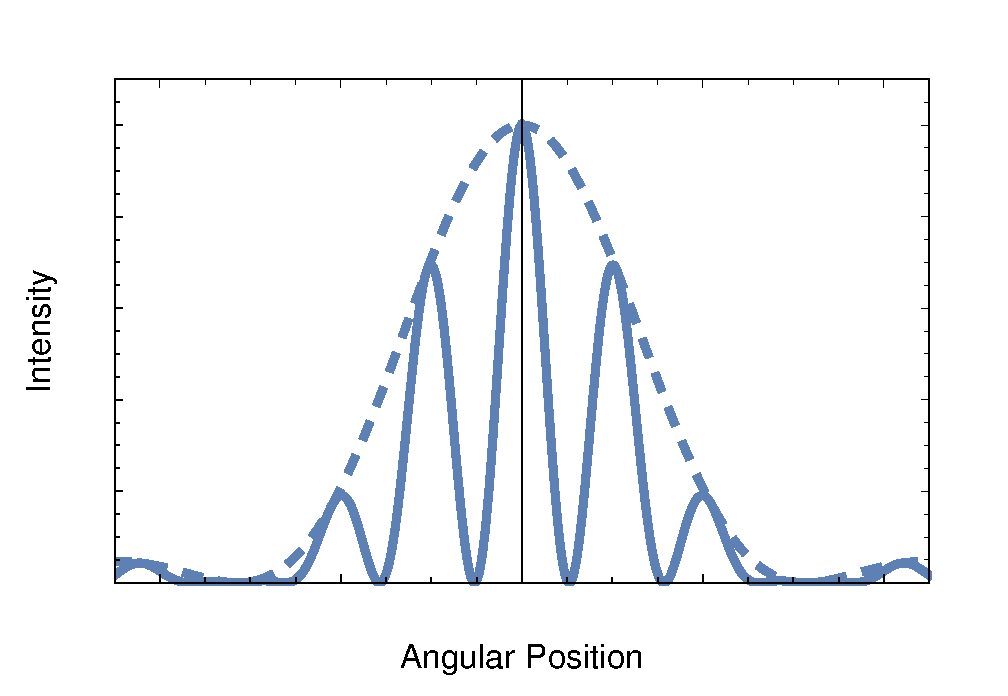
\includegraphics[height=2.75in]{diffraction/diffractionFig3.eps} \par}
\index{color page}
\vspace{0.1cm}

{\centering \textbf{Fig. 4}. Intensity distribution of light passing
through a pair of slits.\par}

The intensity of the interference peaks is no longer constant, but
is modulated by the diffraction envelope represented by the dashed
curve. This dashed curve is a plot of Equation 2 scaled
to the maximum intensity at zero degrees. The intensity of each peak
in the distribution represents the intensity due to the diffraction
effects.  In Activity 1 you recorded the peak position and intensity
for the combined interference{\tt +}diffraction pattern.
We will now use these data to determine the
diffraction pattern and the angular width of the central diffraction
envelope.

%\vspace{5mm}

\textbf{Activity 4: Measuring Diffraction From Double Slit Interference}

(a) Does the intensity distribution you measured in Activity 1 with the phototransistor
resemble the pattern shown in Figure 4? If not, consult your instructor.
\vspace{10mm}

(b) In Activity 1 you recorded the position and intensity of the interference
peaks you measured with the phototransistor. How would you calculate
the angular position of each peak relative to the central maximum?
A sketch might be helpful here.
\vspace{30mm}

(c) Use your expression to calculate the angular position of each
interference peak that you recorded and enter your results in the
table below or in your Excel spreadsheet. Plot intensity versus angular position.
Does your plot resemble the shape of the diffraction pattern you measured in
Activity 2 and shown
in Figure 3? If not, consult your instructor. Print the plot and attach
it to this unit.

\vspace{0.3cm}
{\centering \begin{tabular}{|c|c|}
\hline 
Angular Position (radians)&
Intensity Reading (V)\\
\hline
\hline
&
\\
\hline 
&
\\
\hline 
&
\\
\hline 
&
\\
\hline 
&
\\
\hline 
&
\\
\hline 
&
\\
\hline 
&
\\
\hline 
&
\\
\hline
\end{tabular}\par}
\vspace{0.3cm}

(d) What is the angular width of the central maximum in your data?
Compare this with the measurement you made in Activity 2.
What is your percent difference?
\vspace{25mm}

(e) Collect the results for the angular width from the other teams in class
for this activity and calculate the average and standard deviation. Record the result here.
Are your results consistent with the class results? Why or why not?
\vspace{30mm}

(f) The size of the openings (the slit size $a$) for your single slit and double slit
measurements were the same so the angular width should be the same. Do your data agree?
Does the class data for the two measurements agree?
\vspace{20mm}

(g) How would you explain the difference between the intensity patterns
in Figure 2 and your measurements in Activity 1?
\vspace{20mm}

